\chapter{Software und Datenverarbeitung \(Grote\)}

\section{SensorConnect \(Grote\)}
Im Rahmen dieses Projekts wird die Software SensorConnect zur Erfassung und Analyse von Sensordaten eingesetzt. SensorConnect ist eine Anwendung, die speziell für die Verarbeitung von Messwerten aus Dehnungsmessstreifen (DMS), Kraftsensoren und anderen präzisen Messsystemen konzipiert wurde. Sie bietet eine benutzerfreundliche Oberfläche, mit der Sensordaten in Echtzeit erfasst, visualisiert und analysiert werden können. Ein wesentliches Merkmal von SensorConnect ist die Echtzeit-Datenvisualisierung, die eine unmittelbare Überprüfung der Messwerte ermöglicht. Dies ist besonders in Anwendungen mit dynamischen Lasten oder schnellen Veränderungen der Messgrößen von Vorteil. Zudem erlaubt die Software die Speicherung der erfassten Daten zur späteren Auswertung, was eine detaillierte Analyse und Nachbearbeitung ermöglicht. Die Konfiguration der Sensoren erfolgt über eine intuitive Benutzeroberfläche, die eine schnelle Einrichtung und Kalibrierung ermöglicht. Die Software unterstützt Mehrkanal-Messungen, wodurch mehrere Sensoren gleichzeitig überwacht werden können. Dies ist insbesondere in komplexen Messaufbauten von großer Bedeutung. Darüber hinaus können benutzerdefinierte Schwellenwerte und Alarme eingestellt werden, um Grenzwertüberschreitungen frühzeitig zu erkennen. Ein weiterer Vorteil von SensorConnect ist die Flexibilität beim Export der Messdaten. Die erfassten Werte lassen sich in verschiedenen Formaten, wie CSV oder Excel, speichern und zur Weiterverarbeitung in anderen Softwarelösungen, wie zum Besipiel nCode, verwenden. Dadurch wird eine nahtlose Integration in bestehende Analyseprozesse ermöglicht. Aufgrund dieser Eigenschaften eignet sich SensorConnect besonders für wissenschaftliche und industrielle Anwendungen, in denen präzise Messungen erforderlich sind. Im Rahmen dieses Projekts wird die Software verwendet, um die Sensordaten effizient zu erfassen und zu analysieren, wodurch eine detaillierte Untersuchung der relevanten Messgrößen ermöglicht wird.

\subsection{Installation und Einrichtung}
Die Installation und Einrichtung der SensorConnect-Software war der erste Schritt, um die Messdaten von den Sensoren zu erfassen und analysieren zu können. Im Folgenden werden die notwendigen Schritte zur Installation und Konfiguration beschrieben:

\begin{enumerate}
    \item \textbf{Download der Software}: Besuch der offiziellen Website \footcite{https://www.microstrain.com/software/sensorconnect} von SensorConnect und herunterladen der neuesten Version der Software.
    \item \textbf{Installation}: Ausführen des Installationsprogramm und befolgen der Installationsanweisungen auf dem Bildschirm. Hierbei muss insbesondere sichergestellt werden, dass alle für die Messungen erforderlichen Komponenten installiert werden.
    \item \textbf{Erstkonfiguration}: Starten der Software und ausführen der Erstkonfiguration. Dies umfasst die Einrichtung der Benutzeroberfläche, die Konfiguration der Sensorverbindungen und die Anpassung der Softwareeinstellungen an Ihre spezifischen Anforderungen.
    \item \textbf{Firmware-Updates}: Vor der ersten Benutzung und dem Ausführen von Funktionstests wurde die Firmware der drei Geräte aktualisiert, um sicherzustellen, dass sie mit der neuesten Softwareversion kompatibel sind.
    \item \textbf{Datenspeicher}: SensorConnect speichert die Daten und Konfiguarationen der Sensoren in einem speziellen Ordner, welcher bei Bedarf angepasst werden kann. Es ist ratsam, diesen Ordner regelmäßig zu sichern, um Datenverlust zu vermeiden.
\end{enumerate}

\subsection{Verbindung mit Sensoren}
Nach der Installation und Einrichtung der Software ist der nächste Schritt die Verbindung mit den Sensoren. SensorConnect unterstützt eine Vielzahl von Sensoren und bietet eine benutzerfreundliche Oberfläche zur Verwaltung der Verbindungen. Für unser Projekt wurden uns zwei Sensorknoten vom Typ V-Link-200 zur Verfügung gestellt, welche über einen USB-Stick mit einem Computer verbunden werden können. Die folgenden Schritte beschreiben, wie die Sensoren mit der Software verbunden werden:

\begin{enumerate}
    \item \textbf{Sensoren einschalten}: Vor dem Verbinden mit der Software müssen die Sensoren eingeschaltet und betriebsbereit sein. Dies erfolgt durch Drücken des Ein-/Ausschalters an den Sensorknoten.
    \item \textbf{USB-Stick anschließen}: Anschließen des USB-Sticks an den Computer, um die Verbindung zwischen den Sensoren und der Software herzustellen. Der USB-Stick dient als Schnittstelle zwischen den Sensoren und dem Computer.
    \item \textbf{Sensoren erkennen}: Öffnen von SensorConnect und Aufrufen des Menüpunkts "Devices". Die Software sollte die angeschlossenen Sensoren automatisch erkennen.
    \item \textbf{Sensoren konfigurieren}: Auswählen der erkannten Sensoren und Konfiguration der Sensoreinstellungen, wie z.B. Abtastrate, Messbereich und Kalibrierungsparameter.
    \item \textbf{Verbindung testen}: Ausführen eines Verbindungstests, um sicherzustellen, dass die Sensoren korrekt mit der Software kommunizieren. Dies umfasst das Senden von Testbefehlen an die Sensoren und das Überprüfen der Antwortzeiten.
    \item \textbf{Sensoren kalibrieren}: Kalibrieren der Sensoren, um sicherzustellen, dass die Messwerte präzise und zuverlässig sind. Die Kalibrierung sollte regelmäßig durchgeführt werden, um die Genauigkeit der Messungen zu gewährleisten.
    \item \textbf{Sensoren überwachen}: Überwachen der Sensoren in Echtzeit über die Benutzeroberfläche von SensorConnect, um sicherzustellen, dass die Messwerte stabil und konsistent sind.
\end{enumerate}

\subsection{Datenaufzeichnung und Live-Datenübertragung}
SensorConnect bietet die Möglichkeit, Sensordaten in Echtzeit zu erfassen und aufzuzeichnen. Dies ermöglicht eine kontinuierliche Überwachung der Messwerte und eine detaillierte Analyse der Daten. Die folgenden Schritte beschreiben, wie die Datenaufzeichnung und Live-Datenübertragung durchgeführt werden können:

\begin{enumerate}
    \item \textbf{Aufzeichnungsparameter festlegen}: Festlegen der Parameter für die Datenaufzeichnung, wie zum Beispiel die Dauer der Aufzeichnung, die Abtastrate und das Speicherformat.
    \item \textbf{Aufzeichnung starten}: Starten der Datenaufzeichnung durch Klicken auf die Schaltfläche "Sample".
    \item \textbf{Einstellen der Messparameter}: Auswählen der zu erfassenden Kanäle und Festlegen der Abtastrate. Hier wird ebenfalls eingestellt, ob die Daten nur im internen Speicher des Sensors gespeichert und/oder an den Computer übertragen werden sollen.
    \item \textbf{Aufzeichnung überwachen}: Überwachen des Fortschritts der Datenaufzeichnung in Echtzeit über die Benutzeroberfläche von SensorConnect.
    \item \textbf{Aufzeichnung beenden}: Beenden der Datenaufzeichnung durch Zurücksetzen des Sensors in den Leerlauf. Die erfassten Daten werden automatisch gespeichert.
    \item \textbf{Sensoren speichern}: Die Sensorkonfiguration wird bis zur nächsten Messung gespeichert, um eine schnelle Wiederverwendung zu ermöglichen. Sollten verschiedene Konfigurationen benötigt werden, können diese unabhängig voneinander in verschiedenen Dateien gespeichert und bei Bedarf geladen werden.
\end{enumerate}

\subsection{Datenanalyse}
Nach der Datenaufzeichnung bietet SensorConnect leistungsstarke Werkzeuge zur Analyse der erfassten Daten. Die folgenden Schritte beschreiben, wie eine Datenanalyse durchführt werden kann:

\begin{enumerate}
    \item \textbf{Beenden der Messaufzeichnung}: Beenden der Messaufzeichnung und laden der erfassten Daten in die Software.
    \item \textbf{Analysewerkzeuge auswählen}: Auswahl der gewünschten Analysewerkzeuge, wie zum Beispiel statistische Auswertungen, Frequenzanalysen oder Zeitreihenanalysen.
    \item \textbf{Daten analysieren}: Ausführen der Analyse und Interpretation der Ergebnisse. SensorConnect bietet umfangreiche Visualisierungsmöglichkeiten, um die Analyseergebnisse anschaulich darzustellen.
    \item \textbf{Ergebnisse speichern}: Speichern der Analyseergebnisse und erstellen von Berichten oder Präsentationen.
\end{enumerate}

\subsection{Datenexport}
SensorConnect ermöglicht den Export der erfassten und analysierten Daten in verschiedene Formate, um die Weiterverarbeitung oder Archivierung zu erleichtern. Die folgenden Schritte beschreiben den Datenexport:

\begin{enumerate}
    \item \textbf{Daten auswählen}: Auswahl der Daten, die exportiert werden sollen. Es können entweder die gesamten Daten oder nur bestimmte Datensätze exportiert werden.
    \item \textbf{Export durchführen}: Durchführen des Exports und Speicherung der exportierten Dateien an einem gewünschten Speicherort.
    \item \textbf{Export überprüfen}: Überprüfen der exportierten Dateien, um sicherzustellen, dass alle Daten korrekt und vollständig exportiert wurden.
\end{enumerate}

\subsection{Darstellung und Visualisierung der Messwerte}
Zur besseren Vorstellung der Möglichkeiten von SensorConnect, wird im Folgenden ein Beispiel für die Darstellung und Visualisierung von Messwerten gegeben. Die Software bietet eine Vielzahl von Werkzeugen zur Visualisierung von Sensordaten, die es ermöglichen, die Messwerte in Echtzeit zu überwachen und detaillierte Analysen durchzuführen. Das folgende Beispiel zeigt, wie die Messwerte in verschiedenen Formaten dargestellt werden können:

\begin{figure}[h]
    \begin{center}
        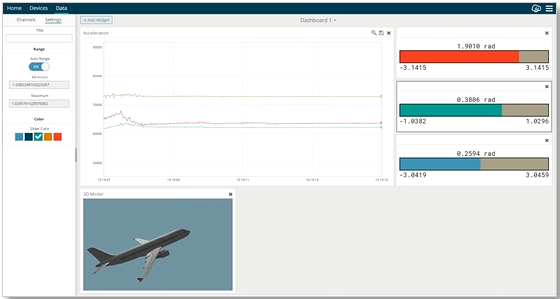
\includegraphics[width=1\textwidth, keepaspectratio]{SensorConnect.png}
        \caption[Benutzeroberfläche in SensorConnect]{SensorConnect
        }
        \label{fig:SensorConnect}
    \end{center}
\end{figure}



\section{nCode \(Grote\)}
Im Rahmen dieses Projekts wird die Software nCode zur Erfassung, Analyse und Auswertung von Messdaten eingesetzt. nCode ist eine leistungsfähige Softwarelösung, die speziell für die Lebensdaueranalyse, Belastungsdatenauswertung und Signalverarbeitung entwickelt wurde. Sie wird häufig in den Bereichen Fahrzeugtechnik, Maschinenbau, Luft- und Raumfahrt sowie strukturelle Überwachung eingesetzt, um Daten aus realen Tests oder Simulationen effizient auszuwerten.
Ein zentraler Vorteil von nCode ist die umfassende Unterstützung für verschiedene Sensordaten, darunter Dehnung, Beschleunigung, Temperatur und andere physikalische Größen. Die Software bietet leistungsfähige Werkzeuge zur Datenfilterung, Signalanalyse und Ermüdungsbewertung, wodurch es möglich ist, kritische Belastungen und potenzielle Schwachstellen in Bauteilen zu identifizieren.
Die intuitive Benutzeroberfläche von nCode erleichtert die Datenaufbereitung und Automatisierung von Analyseprozessen. Dank der Möglichkeit, Python-Skripte und benutzerdefinierte Workflows zu integrieren, kann die Software flexibel an spezifische Anforderungen angepasst werden. Darüber hinaus unterstützt sie eine Vielzahl an Dateiformaten, sodass Messdaten aus verschiedenen Quellen problemlos verarbeitet werden können.
Durch den Einsatz von nCode in diesem Projekt können große Mengen an Sensordaten systematisch analysiert und relevante Erkenntnisse zur Beanspruchung und Lebensdauer von Bauteilen gewonnen werden. Dies trägt dazu bei, fundierte Entscheidungen zur Optimierung und Sicherheit von Konstruktionen zu treffen und die Effizienz der Entwicklungsprozesse zu steigern.
\subsection{Installation und Einrichtung}
Die Installation und Einrichtung der nCode-Software war der erste Schritt, um die Messdaten zu verarbeiten und zu analysieren. Im Folgenden werden die notwendigen Schritte zur Installation und Konfiguration beschrieben:

\begin{enumerate}
    \item \textbf{Download der Software}: Besuch der  Website \footcite{https://wiki.unibw.de/pages/viewpage.action?pageId=103779828} und Herunterladen der neuesten Version von nCode über die Universität.
    \item \textbf{Installation}: Ausführen des Installationsprogramms und Befolgen der Installationsanweisungen auf dem Bildschirm. Hierbei muss insbesondere sichergestellt werden, dass alle für die Datenverarbeitung erforderlichen Komponenten installiert werden.
    \item \textbf{Erstkonfiguration}: Starten der Software und Ausführen der Erstkonfiguration. Dies umfasst die Einrichtung der Benutzeroberfläche, die Konfiguration der Datenverbindungen und die Anpassung der Softwareeinstellungen an Ihre spezifischen Anforderungen.
    \item \textbf{Lizenzierung}: Aktivieren der Softwarelizenz, um alle Funktionen der nCode-Software nutzen zu können.
\end{enumerate}

\subsection{Import von Daten}
Nach der Installation und Einrichtung der Software ist der nächste Schritt der Import der Sensordaten. Die folgenden Schritte beschreiben, wie die Daten in die Software importiert werden:

\begin{enumerate}
    \item \textbf{Datenquelle auswählen}: Auswahl der Datenquelle, aus der die Sensordaten importiert werden sollen, z.B. CSV-Dateien, Excel-Dateien oder Datenbanken.
    \item \textbf{Daten importieren}: Importieren der ausgewählten Daten in die nCode-Software. Die Software bietet verschiedene Importoptionen, um den Prozess zu erleichtern. Hierbei muss insbesondere darauf geachtet werden, dass bei der Kanalauswahl die richtigen Sensorkanäle ausgewählt werden.
    \item \textbf{Daten überprüfen}: Überprüfen der importierten Daten, um sicherzustellen, dass alle Daten korrekt und vollständig importiert wurden.
    \item \textbf{Datenbereinigung}: Bereinigen der Daten, um fehlerhafte oder unvollständige Datensätze zu entfernen. Dies umfasst das Filtern von Ausreißern, das Auffüllen fehlender Werte und das Korrigieren von Messfehlern.
\end{enumerate}

\subsection{Einlesen und Verarbeiten der Daten und die anschließende Ausgabe}
Nach dem Import der Sensordaten bietet nCode leistungsstarke Werkzeuge zur Verarbeitung und Analyse der Daten. Die folgenden Schritte beschreiben, wie die Daten eingelesen und verarbeitet werden können:

\begin{enumerate}
    \item \textbf{Einfügen der Zeitreihe}: Einfügen der importierten Zeitreihendaten in die nCode-Software. Die Software bietet verschiedene Werkzeuge zur Datenvisualisierung und -analyse, um die Daten effizient zu verarbeiten.
    \item \textbf{Auswahl der erforderlichen Werkzeuge}: Für jede Datenauswertung und -analyse stehen verschiedene Werkzeuge zur Verfügung, die je nach Anforderung ausgewählt werden können.
    \item \textbf{Daten verarbeiten}: Verarbeiten der Daten mit den integrierten Werkzeugen zur Signalanalyse, wie z.B. Filterung, Glättung und Interpolation. Dies ermöglicht eine detaillierte Untersuchung der Messwerte und die Identifizierung von relevanten Informationen.
    \item \textbf{Daten analysieren}: Ausführen von Analysen, um Muster, Trends und Anomalien in den Daten zu identifizieren. Die Software bietet verschiedene Analysewerkzeuge, wie z.B. statistische Auswertungen, Frequenzanalysen und Zeitreihenanalysen.
    \item \textbf{Ergebnisse überprüfen}: Überprüfen der Analyseergebnisse, um sicherzustellen, dass alle relevanten Informationen korrekt und vollständig erfasst wurden.   
\end{enumerate}

\section{Darstellung und Visualisierung der Messwerte}
Zur besseren Vorstellung der Möglichkeiten von nCode, wird im Folgenden ein Beispiel für die Darstellung und Visualisierung von Messwerten gegeben. Die Software bietet eine Vielzahl von Werkzeugen zur Visualisierung von Sensordaten, die es ermöglichen, die Messwerte in Echtzeit zu überwachen und detaillierte Analysen durchzuführen. Das folgende Beispiel zeigt, wie man eventuelle Spikes, welche während einer Messung aufgetreten sind, identifizieren und herausfiltern kann:

\begin{figure}[h]
    \begin{center}
        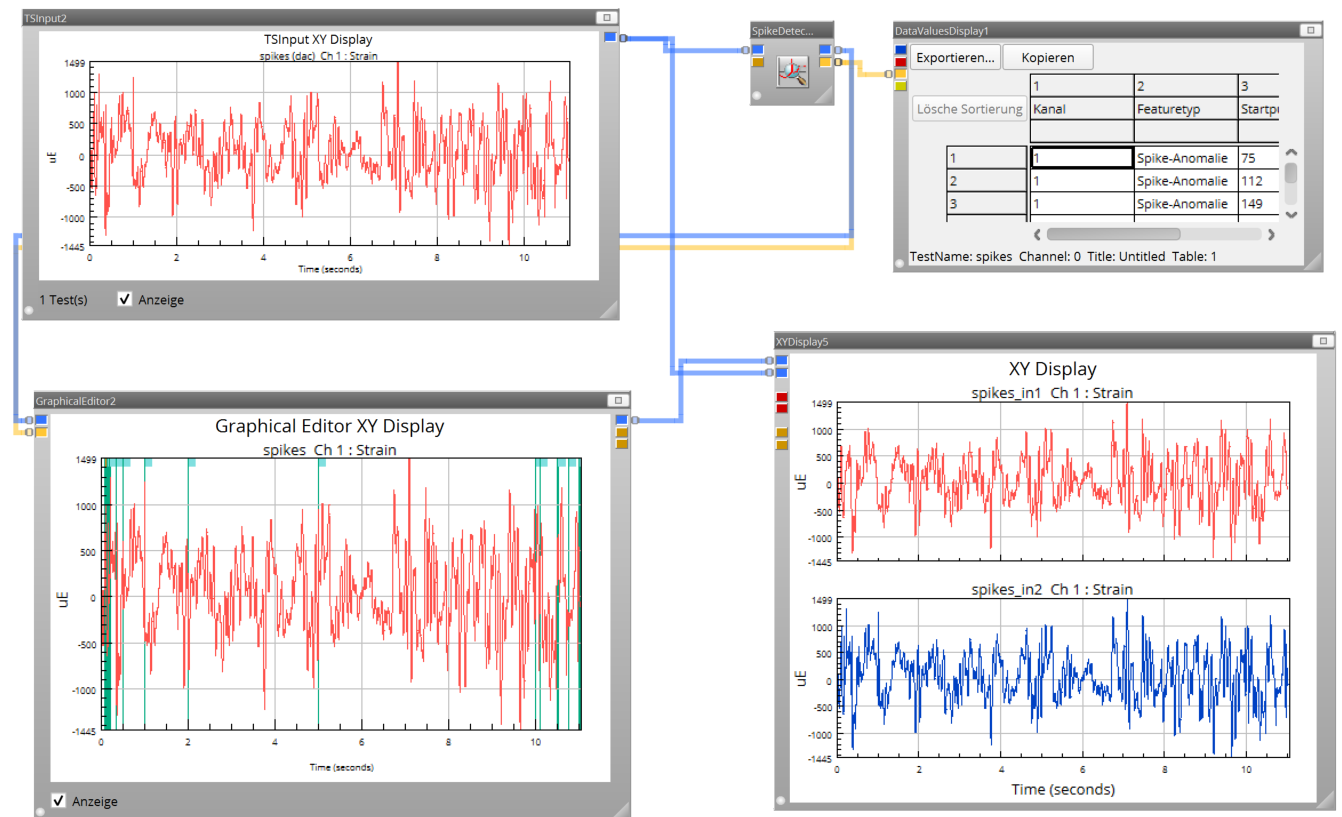
\includegraphics[width=1\textwidth, keepaspectratio]{Spike.png}
        \caption[Spike Detection in nCode]{Spike Detection
        }
        \label{fig:Spike}
    \end{center}
\end{figure}